\documentclass[handout]{beamer}
\usepackage[utf8]{inputenc}
\usepackage[T2A]{fontenc}
\usepackage[english]{babel}
\usepackage{graphicx}
\usepackage{array}
\usetheme{Warsaw}
\usecolortheme{wolverine}

\usepackage{fontawesome5}
\usepackage{listings}
\usepackage[all]{xy}
\usepackage{changepage}

\lstset{
  language=Haskell,
  showstringspaces=false,
  columns=flexible,
  basicstyle={\ttfamily},
  numbers=none,
  numberstyle=\tiny\color{gray},
  keywordstyle=\color{blue},
  commentstyle=\color{dkgreen},
  stringstyle=\color{red},
  breaklines=true,
  breakatwhitespace=true,
  tabsize=2
}

\def\N{\mathbb{N}}

\title[Backtracking, Interleaving, and Terminating Monad\ldots]{Backtracking, Interleaving, and Terminating Monad Transformers}
\author[Andrew Lelechenko]{Andrew Lelechenko \\ \texttt{1@dxdy.ru}}
\institute[Barclays]{Barclays, London}
\date{Papers We Love, London, 29.10.2019}

\begin{document}

\begin{frame}
  \titlepage
\end{frame}


\begin{frame}
\begin{figure}[H]
\centering
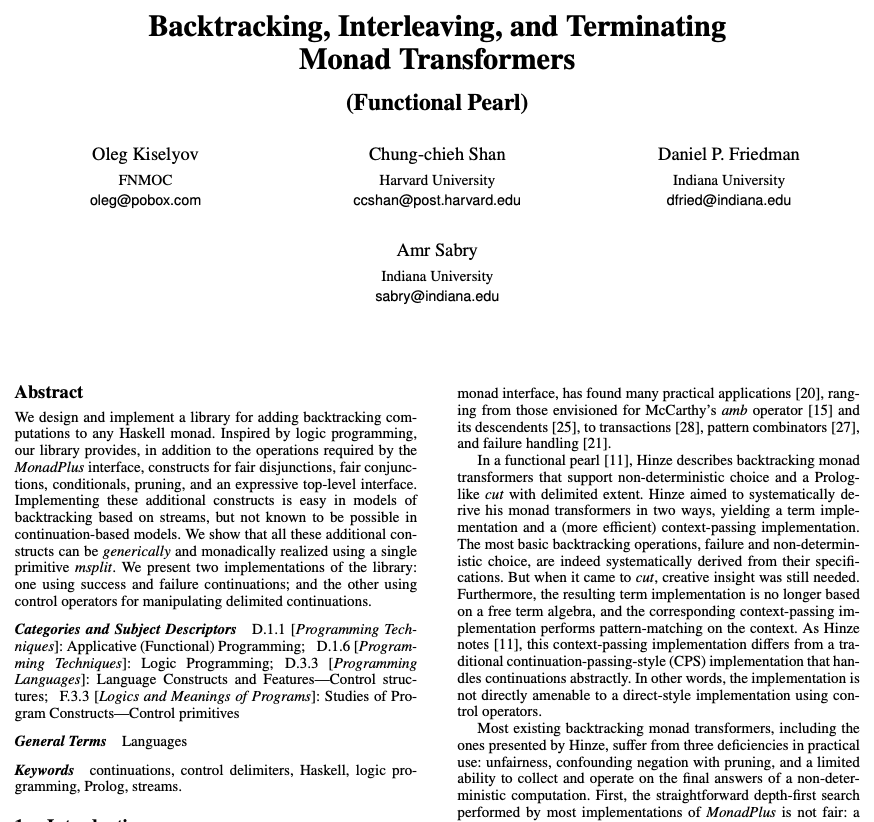
\includegraphics[width=0.9\textwidth]{paper.png}
\end{figure}
\end{frame}

\title{Better List Monad}

\begin{frame}
\begin{figure}[H]
\centering
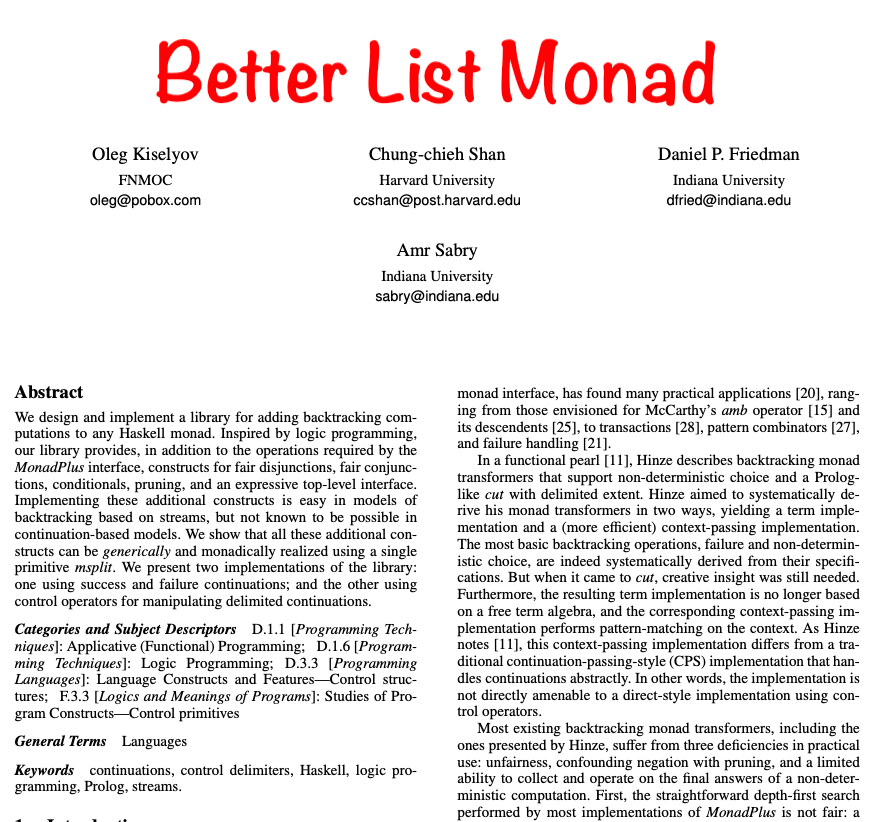
\includegraphics[width=0.9\textwidth]{better-list-monad.png}
\end{figure}
\end{frame}

\title{Better list comprehensions}

\begin{frame}
\begin{figure}[H]
\centering

\includegraphics[width=0.9\textwidth]{better-list-comprehensions.png}
\end{figure}
\end{frame}


\begin{frame}[fragile]{List comprehension}

\vspace{-1.4ex}

\begin{itemize}[<+->]

\item Mathematics:
\begin{multline*}
\{ (x, y) \mid x \in [1,3], y \in [x,4], x + y \le 5 \}
= \\ =
\{ (1, 1), (1, 2), (1, 3), (1, 4), (2, 2), (2, 3) \}.
\end{multline*}

\item Haskell:
\begin{lstlisting}[language=Haskell]
[ (x, y) | x <- [1..3], y <- [x..4], x + y <= 5 ]
\end{lstlisting}

\item Python:
\begin{lstlisting}[language=Python]
{ (x, y)
  for x in range(1, 3)
  for y in range(x, 4)
  if x + y <= 5 }
\end{lstlisting}

\item PostgreSQL:
\begin{lstlisting}[language=SQL]
SELECT x, y
FROM  GENERATE_SERIES(1, 3) AS x,
      GENERATE_SERIES(x, 4) AS y
WHERE x + y <= 5;
\end{lstlisting}

\end{itemize}

\end{frame}

\begin{frame}[fragile]{Infinite lists and $\cup$}
\begin{adjustwidth}{-1em}{-1em}

\begin{itemize}[<+->]

\item Mathematics:
$$ \{ x \mid x \in 2\N, x \equiv 0 \!\!\! \pmod 3 \} = \{ 0, 6, 12\ldots \}.$$

\item Haskell:
\begin{lstlisting}[language=Haskell]
[ x | x <- [0, 2..], x `mod` 3 == 0 ]
\end{lstlisting}

\item Mathematics:
$$ \{ x \mid x \in 2\N \cup 3\N, x \equiv 1 \!\!\! \pmod 2 \} = \{ 3, 9, 15\ldots \}.$$

\item Haskell:
\begin{lstlisting}[language=Haskell]
[ x | x <- [0, 2..] ++ [0, 3..], x `mod` 2 == 1 ]
\end{lstlisting}

\item But this computation stucks forever! Because {\tt (++)} is {\em left-biased.}

\end{itemize}

\end{adjustwidth}
\end{frame}

\begin{frame}[fragile]{Fair interleave aka unbiased $+\!\!+$}

{\tt interleave [0,2,4] [1,3,5,7,9] = [0,1,2,3,4,5,7,9] }

\bigskip

\pause

Simple implementation:
\begin{lstlisting}[language=Haskell]
interleave :: [a] -> [a] -> [a]
interleave [] ys = ys
interleave xs [] = xs
interleave (x:xs) (y:ys) = x : y : interleave xs ys
\end{lstlisting}

\pause

Simple{\bf r} implementation:
\begin{lstlisting}[language=Haskell]
interleave :: [a] -> [a] -> [a]
interleave [] ys = ys
interleave (x:xs) ys = x : interleave ys xs
\end{lstlisting}

\pause

{\bf Bonus level:}
is {\tt interleave} associative?

\end{frame}

\begin{frame}[fragile]{Infinite lists and $\times$}
\begin{adjustwidth}{-1em}{-1em}

\begin{itemize}[<+->]

\item Mathematics:
$$ \{ (x, y) \mid x \in \N, y \in \N, x > y \} $$

\item Haskell:
\begin{lstlisting}[language=Haskell]
[ (x, y) | x <- [0..], y <- [0..], x > y ]
\end{lstlisting}

\item But this computation stucks forever! Imagine it as two nested loops:

\begin{lstlisting}[language=C]
for(int x = 0; ; x++)
  for(int y = 0; ; y++)
    if(x > y)
      printf("(%d, %d)", x, y);
\end{lstlisting}

\end{itemize}

\end{adjustwidth}
\end{frame}

\begin{frame}[fragile]{Unfair interweave aka simplified $\gg\!\!=$}

\begin{lstlisting}[language=Haskell]
interweave :: [a] -> [b] -> [(a, b)]
interweave [] ys = []
interweave (x:xs) ys =
  map (\y -> (x, y)) ys ++ interweave xs ys
\end{lstlisting}

$$\xymatrix{
0,0 \ar[r] & 0,1 \ar[r] & 0,2 \ar[r] & 0,3 \ar[r] & \cdots \ar[dllll] \\
1,0 \ar[r] & 1,1 \ar[r] & 1,2 \ar[r] & 1,3 \ar[r] & \cdots \ar[dllll] \\
2,0 \ar[r] & 2,1 \ar[r] & 2,2 \ar[r] & 2,3 \ar[r] & \cdots \ar[dllll] \\
3,0 \ar[r] & 3,1 \ar[r] & 3,2 \ar[r] & 3,3 \ar[r] & \cdots \\
}$$

\end{frame}

\begin{frame}[fragile]{Fair interweave aka simplified $\gg\!\!-$}

\begin{lstlisting}[language=Haskell]
interweave :: [a] -> [b] -> [(a, b)]
interweave [] ys = []
interweave (x:xs) ys =
  map (\y -> (x, y)) ys `interleave` interweave xs ys
\end{lstlisting}

$$\xymatrix{
0,0 \ar[d]              & 0,1 \ar[ddl]     & 0,2 \ar[dl]  & 0,3 \ar@/_1.4pc/[dddlll] & 0,4 \ar@/_0.5pc/[dll] & 0,5 \ar@/_1pc/[ddllll] & 0,6 \ar@/_0.5pc/[dlll] & \cdots \ar@/_0.5pc/[dlll] \ar@/_0.2pc/[ddlllll] \ar[dll] \ar@/^0.6pc/[dddllllll] \\
1,0 \ar[ur]             & 1,1 \ar@/^0.5pc/[urr]     & 1,2 \ar@/^0.5pc/[urrr] & 1,3 \ar@/^0.5pc/[urrrr]       & 1,4 \ar@/^0.2pc/[urrr] & 1,5 \ar@/_0.2pc/[urr] & \cdots \\
2,0 \ar@/^1pc/[uurr]    & 2,1 \ar@/^1.3pc/[uurrrrr]   & 2,2 \ar[uurrrrr]  & \cdots \\
3,0 \ar@/^2pc/[uuurrrr] & 3,1 \ar@/_0.9pc/[uuurrrrrr] & \cdots \\
}$$

\end{frame}

\begin{frame}[fragile]{Quantifier $\exists$}
\begin{adjustwidth}{-1em}{-1em}

An integer is called {\em composite} if it has at least one non-trivial divisor (other than 1 and itself). E. g., 4 is the smallest composite.

\bigskip

$ \{ x \mid x \in [2, 10], \exists y \in [2, x-1] \,\, x \equiv 0 \pmod y \} =
\{ 4,6,8,9,10 \}$.

\bigskip

\pause

It is not easily expressible in Haskell:
\begin{lstlisting}[language=Haskell]
> [(x, y) | x <- [2..10], y <- [2..x-1], x `mod` y == 0]
[(4,2),(6,2),(6,3),(8,2),(8,4),(9,3),(10,2),(10,5)]
\end{lstlisting}

\pause

\begin{lstlisting}[language=Haskell]
> [x | x <- [2..10], y <- [2..x-1], x `mod` y == 0]
[4,6,6,8,8,9,10,10]
\end{lstlisting}

\pause

{\bf Fun fact:} it is perfectly expressible in SQL:
\begin{lstlisting}[language=SQL]
SELECT x
FROM  GENERATE_SERIES(2, 10) AS x,
      GENERATE_SERIES(2, x-1) AS y
WHERE x % y = 0
GROUP BY x;
\end{lstlisting}

\end{adjustwidth}
\end{frame}

\begin{frame}[fragile]{Quantifier $\exists$ and {\tt once}}

$ \{ x \mid x \in [2, 10], \exists y \in [2, x-1] \,\, x \equiv 0 \pmod y \} =
\{ 4,6,8,9,10 \}$.

\bigskip

We can express $\exists$ via {\em nested list comprehensions:}

\begin{lstlisting}[language=Haskell]
[ x | x <- [2..10],
  [ y | y <- [2..x-1], x `mod` y == 0 ] /= []
]
\end{lstlisting}

\pause

{\bf Even better:} introduce {\tt once} to keep track of the evidence of compositeness:

\begin{lstlisting}[language=Haskell]
once :: [a] -> [a]
once [] = []
once (x:_) = [x]

[ (x, y1) | x <- [2..10], y1 <- once
  [ y | y <- [2..x-1], x `mod` y == 0 ]
]
\end{lstlisting}


\end{frame}

\begin{frame}[fragile]{Quantifier $\forall$}

An integer is called {\em prime} if it is divisible only by 1 and itself.

\bigskip

$ \{ x \mid x \in [2, 10], \forall y \in [2, x-1] \,\, x \not\equiv 0 \pmod y \} =
\{ 2,3,5,7 \}$.

\bigskip

\pause

We again need nested list comprehensions to express it in Haskell:
\begin{lstlisting}[language=Haskell]
[ x | x <- [2..10],
  [ y | y <- [2..x-1], x `mod` y == 0 ] == []
]
\end{lstlisting}

\pause

{\bf Fun fact:} it is yet again perfectly expressible in SQL.
\begin{lstlisting}[language=SQL]
SELECT x
FROM GENERATE_SERIES(2, 10) AS x
LEFT JOIN GENERATE_SERIES(2, x-1) AS y ON x % y = 0
WHERE y IS NULL;
\end{lstlisting}

\end{frame}

\begin{frame}[fragile]{Quantifier $\forall$ and {\tt lnot}}

Can we express $\forall$ via $\exists$? Apply De Morgan's law:

\begin{multline*}
\bigl\{ x \mid x \in [2, 10], \forall y \in [2, x-1] \,\, x \not\equiv 0 \!\!\! \pmod y \bigr\} = \\
\bigl\{ x \mid x \in [2, 10], \neg (\exists y \in [2, x-1] \,\, x \equiv 0 \!\!\! \pmod y) \bigr\}.
\end{multline*}

\pause

Introduce {\tt lnot} combinator (logical negation):

\begin{lstlisting}[language=Haskell]
lnot :: [a] -> [()]
lnot [] = [()]
lnot (_:_) = []

[ x  | x <- [2..10], _ <- lnot
  [ y | y <- [2..x-1], x `mod` y == 0 ]
]
\end{lstlisting}

{\bf For alert readers:} the paper uses a more general combinator {\tt ifte}.

\end{frame}

\begin{frame}{What's next?}

\begin{itemize}[<+->]
\item {\tt interleave}, {\tt interweave}, {\tt once} and {\tt lnot}
      form a pretty expressive DSL for backtracking and relational (logic) programming
      on lists.
\item How to generalize this notion to other data types?
\begin{itemize}
  \item Infinite streams.
  \item Probability distributions:
        {\tt [CatAlive, CatDead]} \par vs.
        {\tt [(0.7, CatAlive), (0.3, CatDead)]}.
\end{itemize}
\item How to handle side effects?
\begin{itemize}
  \item Read input lists from IO (disk, network, whatever).
  \item Cache intermediate computations.
  \item Track progress and write results.
\end{itemize}
\end{itemize}

\end{frame}

\begin{frame}[fragile]{Back to Kiselyov et al., 2005}

\begin{itemize}[<+->]
\item Introduce a type class {\tt MonadLogic}, consisting of
      {\tt interleave}, {\tt interweave}, {\tt once} and {\tt lnot},
      for an arbitrary {\tt MonadPlus} (not just for lists).
\item Propose laws, allowing equational reasoning
      about relational programming.
\item Express all functions by means of a single combinator {\tt msplit}:
\begin{lstlisting}[language=Haskell]
msplit :: [a] -> [Maybe (a, [a])]
msplit [] = [Nothing]
msplit (x:xs) = [Just (x, xs)]
\end{lstlisting}

\item Explain how to add {\tt MonadLogic} capabilities atop any other {\tt Monad},
      giving rise to {\tt LogicT} monad transformer.

\end{itemize}

\end{frame}

\begin{frame}{Final remarks}

\begin{itemize}[<+->]
\item I happened to maintain a Haskell implementation of {\tt LogicT}
      at hackage.haskell.org/package/logict
\item Modern developments in Haskell and relational programming:
      twitch.tv/ekmett/videos
\item SQL is a logic programming language.
\end{itemize}

\bigskip
\bigskip
\bigskip

\par \faAt\ andrew.lelechenko@gmail.com
\hspace{7.5em}
\faGithub\ \faTelegram\ Bodigrim

\bigskip
\bigskip
\bigskip

\centerline{\Huge\bf Thank you!}
\end{frame}

\end{document}
